%%%%%%%%%%%%%%%%%%%%%%%%%%%%%%%%%%%%%%%%%%%%%%%%%%%%%%%%%%%%%%%%%%%%%%%
%% Hauptdokument
%%%%%%%%%%%%%%%%%%%%%%%%%%%%%%%%%%%%%%%%%%%%%%%%%%%%%%%%%%%%%%%%%%%%%%%

\documentclass[12pt, a4paper, twoside]{exam}
\usepackage{ german,
             %umlaut,
             makeidx,
             amsfonts, epsf,
             amsmath,
             bibgerm,
             epsfig,
             fancyheadings,
             subfigure}
\usepackage[utf8]{inputenc} % set up unicode input
\usepackage[T1]{fontenc} % set 8-bit font enconding
	% see: http://tex.stackexchange.com/questions/664/why-should-i-use-usepackaget1fontenc
\usepackage{paratype} % PTSans - corporate design font of the University of Kaiserslautern
	\renewcommand{\familydefault}{\sfdefault}
\usepackage{wallpaper} % for background image on title page

\usepackage{amsthm,amssymb,longtable,array,bm,varioref,graphicx,url,moreverb,ifthen,mdwlist,icomma}
\usepackage{capt-of}
\usepackage[english]{babel}
\usepackage{layout,ae,float,trsym,trfsigns}
\usepackage[nice]{units}
\usepackage[dvips]{rotating}
\usepackage[dvips]{geometry}
\usepackage{rotating}
\usepackage{lastpage}
%%%%%%%%%%%%%%%%%%%%%%%%%%%%%%%%%%%%%%%%%%%%%%%%%%%%%%%%%%%%%%%%%%%%%%%
%% Formatierungen
%%%%%%%%%%%%%%%%%%%%%%%%%%%%%%%%%%%%%%%%%%%%%%%%%%%%%%%%%%%%%%%%%%%%%%%
\setlength{\parindent}{0cm}
\setlength{\parskip}{2ex}
\setlength{\textwidth}{160mm} \setlength{\topmargin}{-6mm}
\setlength{\textheight}{230mm}

\setlength{\oddsidemargin}{0mm} \setlength{\evensidemargin}{0mm}

\clubpenalty=1000000 \widowpenalty=1000000

%%%%%%%%%%%%%%%%%%%%%%%%%%%%%%%%%%%%%%%%%%%%%%%%%%%%%%%%%%%%%%%%%%%%%%%
%% Template Configuration
%%%%%%%%%%%%%%%%%%%%%%%%%%%%%%%%%%%%%%%%%%%%%%%%%%%%%%%%%%%%%%%%%%%%%%

% LaTeX exam class configuration
\iftoggle{isGerman}{
	\pointpoints{Punkt}{Punkte}
	\qformat{\textbf{\large Aufgabe \thequestion}\quad\textbf{\large(\thepoints)}\hfill\rule[-3ex]{0ex}{3ex}}
	\renewcommand{\solutiontitle}{\noindent\textbf{Lösung:}\par\noindent}
}{
	\pointpoints{point}{points}
	\qformat{\textbf{\large Question \thequestion}\quad\textbf{\large(\thepoints)}\hfill\rule[-3ex]{0ex}{3ex}}
}


%%%%%%%%%%%%%%%%%%%%%%%%%%%%%%%%%%%%%%%%%%%%%%%%%%%%%%%%%%%%%%%%%%%%%%%
%% Global Formatting Settings
%%%%%%%%%%%%%%%%%%%%%%%%%%%%%%%%%%%%%%%%%%%%%%%%%%%%%%%%%%%%%%%%%%%%%%%
\setlength{\parindent}{0cm}
\setlength{\parskip}{2ex}
\setlength{\textwidth}{160mm} \setlength{\topmargin}{-6mm}
\setlength{\textheight}{230mm}

\setlength{\oddsidemargin}{0mm} \setlength{\evensidemargin}{0mm}

\clubpenalty=1000000 \widowpenalty=1000000

% change figure labels to abbreviated versions
\addto\captionsenglish{\renewcommand{\figurename}{Fig.}}


%%%%%%%%%%%%%%%%%%%%%%%%%%%%%%%%%%%%%%%%%%%%%%%%%%%%%%%%%%%%%%%%%%%%%%%
%% Headers & Footers
%%%%%%%%%%%%%%%%%%%%%%%%%%%%%%%%%%%%%%%%%%%%%%%%%%%%%%%%%%%%%%%%%%%%%%%

% page style for front page
\fancypagestyle{frontpage}{
	\fancyhf{}
	
	%remove top line
	\renewcommand{\headrulewidth}{0pt}

	\fancyfoot[L]{
		\color{tuk-coldgrey} \pt \footnotesize
		\examID~\examTitleShort
	}
	\fancyfoot[C]{
		\color{tuk-coldgrey} \pt \footnotesize
		\examPeriod
	}
	\fancyfoot[R]{
		\color{tuk-coldgrey} \pt \footnotesize
		\iftoggle{isGerman}{
  			Seite \thepage\ von \pageref{LastPage}
		}{
			Page \thepage\ of \pageref{LastPage}
		}
	}
}

% page style for all other pages
\fancypagestyle{otherpages}{
	\fancyhf{}

	\fancyhead[L]{
		\iftoggle{isGerman}{
  			Name: \hspace{7cm} Matrikelnummer:
		}{
			Name: \hspace{7cm} Matriculation Number:
		}
	}

	\fancyfoot[L]{
		\color{tuk-coldgrey} \pt \footnotesize
		\examID~\examTitleShort
	}
	\fancyfoot[C]{
		\color{tuk-coldgrey} \pt \footnotesize
		\examPeriod
	}
	\fancyfoot[R]{
		\color{tuk-coldgrey} \pt \footnotesize
		\iftoggle{isGerman}{
  			Seite \thepage\ von \pageref{LastPage}
		}{
			Page \thepage\ of \pageref{LastPage}
		}
	}
}


%%%%%%%%%%%%%%%%%%%%%%%%%%%%%%%%%%%%%%%%%%%%%%%%%%%%%%%%%%%%%%%%%%%%%%%
%% Additional Command Definitions
%%%%%%%%%%%%%%%%%%%%%%%%%%%%%%%%%%%%%%%%%%%%%%%%%%%%%%%%%%%%%%%%%%%%%%%

% AMS operators
\DeclareMathOperator{\sign}{sign}

% points on minor diagonal
\newcommand{\rdots}{\mathinner{
  \mkern1mu\raise1pt\hbox{.}
  \mkern2mu\raise4pt\hbox{.}
  \mkern2mu\raise7pt\vbox{\kern7pt\hbox{.}}\mkern1mu}}

% bold vectors and matrices
\renewcommand{\vec}[1]{\boldsymbol{#1}}

% bold Greek letters
\newcommand{\MB}[1]{{\mbox{\mathversion{bold}$#1$}}}

% matrix with round brackets
\newcommand{\mat}[1]{\begin{pmatrix}#1\end{pmatrix}}

% hints and annotations
\newcommand{\Hinweis}{\textbf{Hinweis:~}}
\newcommand{\Hint}{\textbf{Hint:~}}
\newcommand{\Annotation}{\textbf{Annotation:~}}

% partial derivation with power
% Use: \parfr[<power>]{<nominator>}{<denominator>}
\newcommand{\parfr}[3][\empty]{
	\ifthenelse{\equal{#1}{\empty}}
	{\frac{\partial {#2}}{\partial {#3}}}
	{\frac{\partial^{#1} {#2}}{\partial {#3}^{#1}}}
	}
	
% normal derivation with power
% Use: \dfr[<power>]{<nominator>}{<denominator>}
\newcommand{\dfr}[3][\empty]{
	\ifthenelse{\equal{#1}{\empty}}
	{\frac{\text{d} {#2}}{\text{d} {#3}}}
	{\frac{\text{d}^{#1} {#2}}{\text{d} {#3}^{#1}}}
	}

% number in a circle (in text or formula)
\newcommand{\mycirc}[1]{\mbox{\textcircled{\footnotesize #1}}}

% explicit points notation
\newcommand{\Points}[1]{\text{~\textbf{($\boldsymbol{#1}$~P)}}}

%%%%%%%%%%%%%%%%%%%%%%%%%%%%%%%%%%%%%%%%%%%%%%%%%%%%%%%%%%%%%%%%%%%%%%%
%% Beginn des Dokumentes
%%%%%%%%%%%%%%%%%%%%%%%%%%%%%%%%%%%%%%%%%%%%%%%%%%%%%%%%%%%%%%%%%%%%%%%
\begin{document}

%%%%%%%%%%%%%%%%%%%%%%%%%%%%%%%%%%%%%%%%%%%%%%%%%%%%%%%%%%%%%%%%%%%%%%%
%% Einstellung der FancyHeadings (später durch Koma ersetzen!)
%%%%%%%%%%%%%%%%%%%%%%%%%%%%%%%%%%%%%%%%%%%%%%%%%%%%%%%%%%%%%%%%%%%%%%%
\pagestyle{fancy}

\lhead
   [\sc
   	Exam \pruefungsnummer~\pruefungsnamekurz
   ]
   {\sc
   Name: \hspace{6.5cm} Matriculation Number:}

\rhead
   [\sc
   	\pruefungszeitraum 
 	 ]
   {
   }

%\cfoot{--\hspace{1ex}page \thepage \hspace{1ex}--}
\cfoot{--\hspace{1ex}page \thepage \hspace{1ex}of\hspace{1ex} \pageref{LastPage} \hspace{1ex}--}

%%%%%%%%%%%%%%%%%%%%%%%%%%%%%%%%%%%%%%%%%%%%%%%%%%%%%%%%%%%%%%%%%%%%%%%
%% Deckblatt
%%%%%%%%%%%%%%%%%%%%%%%%%%%%%%%%%%%%%%%%%%%%%%%%%%%%%%%%%%%%%%%%%%%%%%%
%%%%%%%%%%%%%%%%%%%%%%%%%%%%%%%%%%%%%%%%%%%%%%%%%%%%%%%%%%%%%%%%%%%%%%%
%% Front Page
%%%%%%%%%%%%%%%%%%%%%%%%%%%%%%%%%%%%%%%%%%%%%%%%%%%%%%%%%%%%%%%%%%%%%%

% apply front page header and footer settings here
\thispagestyle{frontpage}

% fields for name and matriculation number
\iftoggle{isGerman}{
	Name: \hspace{7cm} Matrikelnummer:
}{
	Name: \hspace{7cm} Matriculation Number:
}\vspace{-10pt}
\\
\rule{\textwidth}{0.5pt}


\begin{center}
	% title and ID
	{\Large\bf\sc
		\iftoggle{isGerman}
		{
			Klausur
		}
		{
			Exam
		}
	\examID\\ in \\
	\examTitleLong \\}\vspace{1.0cm}
	
	% date
	\examDate

\end{center}


%%%%%%%%%%%%%%%%%%%%%%%%%%%%%%%%%%%%%%%%%%%%%%%%%%%%%%%%%%%%%%%%%%%%%%%
%% Exam Regulations
%%%%%%%%%%%%%%%%%%%%%%%%%%%%%%%%%%%%%%%%%%%%%%%%%%%%%%%%%%%%%%%%%%%%%%

\todo{put your own regulations here!}

\underline{Permitted aids:}

Slide-rule or {\bf {non}}programmable calculator, \textbf{maximally 1 handwritten DIN A4 sheet}, dictionaries ({\bf non-electronic}), writing and drawing material.
    
Using non-permitted aids like \textbf{scratch paper}, script, lecture notes, books, copies, programmable calculators or laptops is a deceit and leads to the non-admission of the exam.\\
  
\underline{Please note:}
\begin{enumerate}
	\item Write your \textbf{name} and \textbf{matriculation number} on every sheet.
	\item The calculations and solutions to the problems must be written on the related pages. If the space is not sufficient, further sheets are provided. Solutions on those sheets will be considered 
	      only if there exists a reference to the problem and the solution on the extra sheet is marked correspondingly.
	\item Don't write with a pencil. Don't use red or green color.
	\item {\bf Generally every solution must be proved by calculation or explanation.}
\end{enumerate}
    
\underline{Statement:}

With accepting the exam I declare to be able to participate in the exam \examTitleLong~according to my health status.


%%%%%%%%%%%%%%%%%%%%%%%%%%%%%%%%%%%%%%%%%%%%%%%%%%%%%%%%%%%%%%%%%%%%%%%
%% Punkteberechnung
%%%%%%%%%%%%%%%%%%%%%%%%%%%%%%%%%%%%%%%%%%%%%%%%%%%%%%%%%%%%%%%%%%%%%%%
{\bf\large Evaluation}\\

\begin{center}
	\vqword{Problem}
	\vpword{Achievable points}
	\vsword{Achieved points}
	\cellwidth{2.2em}
	\addpoints
	\gradetable[v]
\end{center}

\begin{table}[h]
	\centering
		\begin{tabular}{|l||c|}
		\hline 
		Total points & \numpoints \\ \hline 
		Achieved points & \hspace{3cm} \\ \hline
		Grade & \\ \hline 
		\end{tabular}
\end{table}

{\bf\large Post-exam review}\\
\begin{table}[h]
	\centering
		\begin{tabular}{*{2}{|l|}}
			\hline
			\textsc{date} &  \\ \hline
			\textsc{signature} & \hspace{4cm} \\ \hline
		\end{tabular}
\end{table}


%%%%%%%%%%%%%%%%%%%%%%%%%%%%%%%%%%%%%%%%%%%%%%%%%%%%%%%%%%%%%%%%%%%%%%%
%% Aufgaben
%%%%%%%%%%%%%%%%%%%%%%%%%%%%%%%%%%%%%%%%%%%%%%%%%%%%%%%%%%%%%%%%%%%%%%%

\begin{questions}
\clearpage

\question[3]
%
\textbf{Logic Gates}

Implement the logic function: $$Z=\overline{(A+B)\cdot(C\cdot D)}$$ You can only
use the logic gates shown in Fig.~\ref{fig:gates}!

\begin{figure}[h]
	\centering
		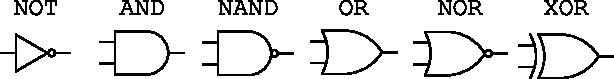
\includegraphics{img/gates.pdf}
	\caption{Available logic gates}
	\label{fig:gates}
\end{figure}

\clearpage

% TODO: Add More tasks here

\end{questions}

\begin{center}
	{\bf\large Correspondence Table}
\end{center}
%
\begin{table}[h!]
\centering
\setlength{\extrarowheight}{0.43cm} 
\begin{tabular}{|c|c|c|} \hline
	No. & $\displaystyle f(t)$ 					& $\displaystyle F(s)$
			\tabularnewline [0.4cm] \hline 
	1   & $\displaystyle \delta(t)$ 		& $\displaystyle 1$
			\tabularnewline [0.4cm] \hline
	2 	& $\displaystyle \sigma(t)$ 		& $\displaystyle \frac{1}{s}$
			\tabularnewline [0.4cm] \hline
	3 	& $\displaystyle t$ 						& $\displaystyle \frac{1}{s^2}$
			\tabularnewline [0.4cm] \hline
	4 	& $\displaystyle \frac{t^2}{2}$ & $\displaystyle \frac{1}{s^3}$
			\tabularnewline [0.4cm] \hline
	5 	& $\displaystyle \frac{t^{n-1}}{(n-1)!}$ & $\displaystyle \frac{1}{s^n}$ 
			\tabularnewline [0.4cm] \hline
	6 	& $\displaystyle e^{-at}$ 			& $\displaystyle \frac{1}{s+a}$
			\tabularnewline [0.4cm] \hline
	7 	& $\displaystyle t e^{-at}$ 		& $\displaystyle \frac{1}{(s+a)^2}$
			\tabularnewline [0.4cm] \hline
	8 	& $\displaystyle t^2 e^{-at}$ 	& $\displaystyle	\frac{2}{(s+a)^3}$
			\tabularnewline [0.4cm] \hline
%	9 	& $\displaystyle 1-e^{-at}$ 		& $\displaystyle \frac{a}{s (s+a)}$
%			\tabularnewline [0.4cm] \hline
%	10  & $\displaystyle \frac{1}{b-a} (e^{-at} - e^{-bt})$ & $\displaystyle \frac{1}{(s+a)(s+b)}$
%			\tabularnewline [0.4cm] \hline
	9 	& $\displaystyle \sin(\omega t)$ & $\displaystyle \frac{\omega}{s^2 + \omega^2}$
			\tabularnewline [0.4cm] \hline
	10 	& $\displaystyle \cos(\omega t)$ & $\displaystyle \frac{s}{s^2 + \omega^2}$
			\tabularnewline [0.4cm] \hline
	11 	& $\displaystyle e^{-at} \sin(\omega t)$ & $\displaystyle \frac{\omega}{(s+a)^2 + \omega^2}$
			\tabularnewline [0.4cm] \hline
	12 	& $\displaystyle e^{-at} \cos(\omega t)$ & $\displaystyle \frac{s+a}{(s+a)^2 + \omega^2}$
			\tabularnewline [0.4cm] \hline
\end{tabular}
\end{table}

%%%%%%%%%%%%%%%%%

\end{document}

%%%%%%%%%%%%%%%%%%%%%%%%%%%%%%%%%%%%%%%%%%%%%%%%%%%%%%%%%%%%%%%%%%%%%%%


